% Part: biographies 
% Chapter: kurt-godel 
% Section: biography
\documentclass[../../../include/open-logic-section]{subfiles}

\begin{document}

\olfileid{bio}{kgd}{bio} 
\olsection{Biography}

\begin{figure}[h!] 
\centering
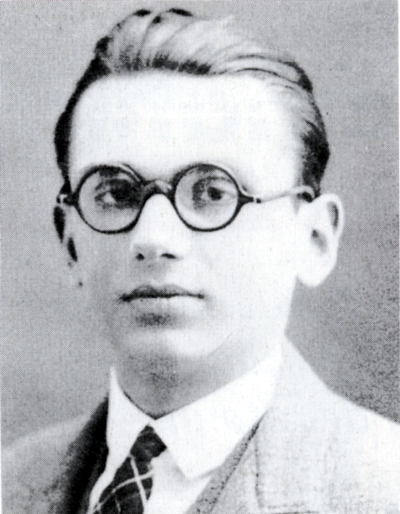
\includegraphics[scale=0.5]{kurt-godel.png} 
\caption{Kurt G{\"o}del. Photo Credit: Wikimedia Commons.} 
\end{figure}

Kurt G{\"o}del was born on April 28, 1906 in Br{\"u}nn in the
Austro-Hungarian empire (now Brno in the Czech Republic). Due to his
inquisitive and bright nature, G{\"o}del was often called ``Der Herr
Warum'' (Mr. Why) by his family~\citep[1]{Dawson1997}. He excelled in
academics since primary school, where he got less than the highest grade
only in mathematics \citep[15]{Dawson1997}. Although he excelled, G{\"o}del was
often absent from school due to poor health and was exempt from physical
education \citep[10]{Dawson1997}. G{\"o}del was diagnosed with rheumatic fever
during his childhood. Throughout his life, he believed this permanently
affected his heart despite medical assessment saying otherwise
\citep[11]{Dawson1997}.

G{\"o}del began studying at the University of Vienna in 1920 and completed his
doctorial studies in 1929. Meaning to study physics, his interests began
moving to the realm of mathematics. His dissertation,
wiritten under the supervision of Hans Hahn, proved the completeness
theorem of first-order predicate logic with identity. Only a couple years
later, his most famous results were published - The first and second
incompleteness theorems~\citep{Godel1931}. During his time in Vienna,
G{\"o}del also became involved with the members of the Vienna Circle.

In 1938 G{\"o}del married his wife, Adele Nimbursky, to his parent's dismay. Not
only was she six years his senior, and a divorcee, but she was employed as
a dancer at a club. At the time in Vienna, marrying a dancer was often
followed by social disgrace \citep[34]{Dawson1997} The social pressures did not
affect G{\"o}del, and they remained happily married until his death.

In 1939, due to political turmoil in Vienna, G{\"o}del and Adele emmigrated to
the United States, where he took up a position at the Institute for
Advanced Study in Princeton, New Jersey. Despite his inroversion and
eccentric nature, G{\"o}del's time at Princeton was collaborative and fruitful.
He published essays in set theory, philosophy and physics. Notably, he
struck up a particularly strong friendship with physicist Albert Einstein
who was also living in the Princeton at the time.

In his later years, G{\"o}del's mental health declined. His wife's frequent
hospitalization in the years leading up to his death meant she was no
longer able to cook his meals for him. Succumbing to both paranoia and
anorexia, and deathly afraid of being poisoned, G{\"o}del refused to eat
\citep[251]{Dawson1997}. He passed away on January 14, 1978 in Princeton.

\end{document}